\PassOptionsToPackage{unicode=true}{hyperref} % options for packages loaded elsewhere
\PassOptionsToPackage{hyphens}{url}
%
\documentclass[ignorenonframetext,]{beamer}
\usepackage{pgfpages}
\setbeamertemplate{caption}[numbered]
\setbeamertemplate{caption label separator}{: }
\setbeamercolor{caption name}{fg=normal text.fg}
\beamertemplatenavigationsymbolsempty
% Prevent slide breaks in the middle of a paragraph:
\widowpenalties 1 10000
\raggedbottom
\setbeamertemplate{part page}{
\centering
\begin{beamercolorbox}[sep=16pt,center]{part title}
  \usebeamerfont{part title}\insertpart\par
\end{beamercolorbox}
}
\setbeamertemplate{section page}{
\centering
\begin{beamercolorbox}[sep=12pt,center]{part title}
  \usebeamerfont{section title}\insertsection\par
\end{beamercolorbox}
}
\setbeamertemplate{subsection page}{
\centering
\begin{beamercolorbox}[sep=8pt,center]{part title}
  \usebeamerfont{subsection title}\insertsubsection\par
\end{beamercolorbox}
}
\AtBeginPart{
  \frame{\partpage}
}
\AtBeginSection{
  \ifbibliography
  \else
    \frame{\sectionpage}
  \fi
}
\AtBeginSubsection{
  \frame{\subsectionpage}
}
\usepackage{lmodern}
\usepackage{amssymb,amsmath}
\usepackage{ifxetex,ifluatex}
\usepackage{fixltx2e} % provides \textsubscript
\ifnum 0\ifxetex 1\fi\ifluatex 1\fi=0 % if pdftex
  \usepackage[T1]{fontenc}
  \usepackage[utf8]{inputenc}
  \usepackage{textcomp} % provides euro and other symbols
\else % if luatex or xelatex
  \usepackage{unicode-math}
  \defaultfontfeatures{Ligatures=TeX,Scale=MatchLowercase}
\fi
\usecolortheme{beaver}
% use upquote if available, for straight quotes in verbatim environments
\IfFileExists{upquote.sty}{\usepackage{upquote}}{}
% use microtype if available
\IfFileExists{microtype.sty}{%
\usepackage[]{microtype}
\UseMicrotypeSet[protrusion]{basicmath} % disable protrusion for tt fonts
}{}
\IfFileExists{parskip.sty}{%
\usepackage{parskip}
}{% else
\setlength{\parindent}{0pt}
\setlength{\parskip}{6pt plus 2pt minus 1pt}
}
\usepackage{hyperref}
\hypersetup{
            pdftitle={Manejo de datos en R (I)},
            pdfauthor={Introducción a la Línea de Comandos para Análisis Bioinformáticos},
            pdfborder={0 0 0},
            breaklinks=true}
\urlstyle{same}  % don't use monospace font for urls
\newif\ifbibliography
\usepackage{color}
\usepackage{fancyvrb}
\newcommand{\VerbBar}{|}
\newcommand{\VERB}{\Verb[commandchars=\\\{\}]}
\DefineVerbatimEnvironment{Highlighting}{Verbatim}{commandchars=\\\{\}}
% Add ',fontsize=\small' for more characters per line
\usepackage{framed}
\definecolor{shadecolor}{RGB}{248,248,248}
\newenvironment{Shaded}{\begin{snugshade}}{\end{snugshade}}
\newcommand{\AlertTok}[1]{\textcolor[rgb]{0.94,0.16,0.16}{#1}}
\newcommand{\AnnotationTok}[1]{\textcolor[rgb]{0.56,0.35,0.01}{\textbf{\textit{#1}}}}
\newcommand{\AttributeTok}[1]{\textcolor[rgb]{0.77,0.63,0.00}{#1}}
\newcommand{\BaseNTok}[1]{\textcolor[rgb]{0.00,0.00,0.81}{#1}}
\newcommand{\BuiltInTok}[1]{#1}
\newcommand{\CharTok}[1]{\textcolor[rgb]{0.31,0.60,0.02}{#1}}
\newcommand{\CommentTok}[1]{\textcolor[rgb]{0.56,0.35,0.01}{\textit{#1}}}
\newcommand{\CommentVarTok}[1]{\textcolor[rgb]{0.56,0.35,0.01}{\textbf{\textit{#1}}}}
\newcommand{\ConstantTok}[1]{\textcolor[rgb]{0.00,0.00,0.00}{#1}}
\newcommand{\ControlFlowTok}[1]{\textcolor[rgb]{0.13,0.29,0.53}{\textbf{#1}}}
\newcommand{\DataTypeTok}[1]{\textcolor[rgb]{0.13,0.29,0.53}{#1}}
\newcommand{\DecValTok}[1]{\textcolor[rgb]{0.00,0.00,0.81}{#1}}
\newcommand{\DocumentationTok}[1]{\textcolor[rgb]{0.56,0.35,0.01}{\textbf{\textit{#1}}}}
\newcommand{\ErrorTok}[1]{\textcolor[rgb]{0.64,0.00,0.00}{\textbf{#1}}}
\newcommand{\ExtensionTok}[1]{#1}
\newcommand{\FloatTok}[1]{\textcolor[rgb]{0.00,0.00,0.81}{#1}}
\newcommand{\FunctionTok}[1]{\textcolor[rgb]{0.00,0.00,0.00}{#1}}
\newcommand{\ImportTok}[1]{#1}
\newcommand{\InformationTok}[1]{\textcolor[rgb]{0.56,0.35,0.01}{\textbf{\textit{#1}}}}
\newcommand{\KeywordTok}[1]{\textcolor[rgb]{0.13,0.29,0.53}{\textbf{#1}}}
\newcommand{\NormalTok}[1]{#1}
\newcommand{\OperatorTok}[1]{\textcolor[rgb]{0.81,0.36,0.00}{\textbf{#1}}}
\newcommand{\OtherTok}[1]{\textcolor[rgb]{0.56,0.35,0.01}{#1}}
\newcommand{\PreprocessorTok}[1]{\textcolor[rgb]{0.56,0.35,0.01}{\textit{#1}}}
\newcommand{\RegionMarkerTok}[1]{#1}
\newcommand{\SpecialCharTok}[1]{\textcolor[rgb]{0.00,0.00,0.00}{#1}}
\newcommand{\SpecialStringTok}[1]{\textcolor[rgb]{0.31,0.60,0.02}{#1}}
\newcommand{\StringTok}[1]{\textcolor[rgb]{0.31,0.60,0.02}{#1}}
\newcommand{\VariableTok}[1]{\textcolor[rgb]{0.00,0.00,0.00}{#1}}
\newcommand{\VerbatimStringTok}[1]{\textcolor[rgb]{0.31,0.60,0.02}{#1}}
\newcommand{\WarningTok}[1]{\textcolor[rgb]{0.56,0.35,0.01}{\textbf{\textit{#1}}}}
\usepackage{graphicx,grffile}
\makeatletter
\def\maxwidth{\ifdim\Gin@nat@width>\linewidth\linewidth\else\Gin@nat@width\fi}
\def\maxheight{\ifdim\Gin@nat@height>\textheight\textheight\else\Gin@nat@height\fi}
\makeatother
% Scale images if necessary, so that they will not overflow the page
% margins by default, and it is still possible to overwrite the defaults
% using explicit options in \includegraphics[width, height, ...]{}
\setkeys{Gin}{width=\maxwidth,height=\maxheight,keepaspectratio}
\setlength{\emergencystretch}{3em}  % prevent overfull lines
\providecommand{\tightlist}{%
  \setlength{\itemsep}{0pt}\setlength{\parskip}{0pt}}
\setcounter{secnumdepth}{0}

% set default figure placement to htbp
\makeatletter
\def\fps@figure{htbp}
\makeatother

\usepackage{tikz}
\usepackage{graphicx}
\usetikzlibrary{calc}
\usepackage{pgfplots}
\usepackage{environ}
\useoutertheme{miniframes}
\useinnertheme{circles}

\title{Manejo de datos en R (I)}
\author{Introducción a la Línea de Comandos para Análisis Bioinformáticos}
\date{02 de Marzo, 2020}

\begin{document}
\frame{\titlepage}

\begin{frame}{Breve repaso}
\protect\hypertarget{breve-repaso}{}

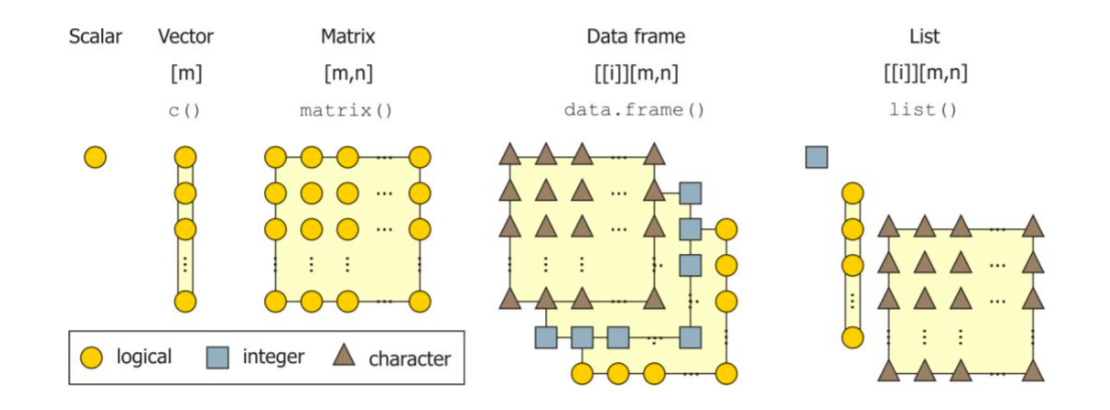
\includegraphics{r_tipos_datos.png}

\href{https://hal.archives-ouvertes.fr/hal-01846155/document}{A
practical guide to the R package Luminescence (Dietze et al., 2013)}

\end{frame}

\begin{frame}{Breve repaso}
\protect\hypertarget{breve-repaso-1}{}

\begin{center}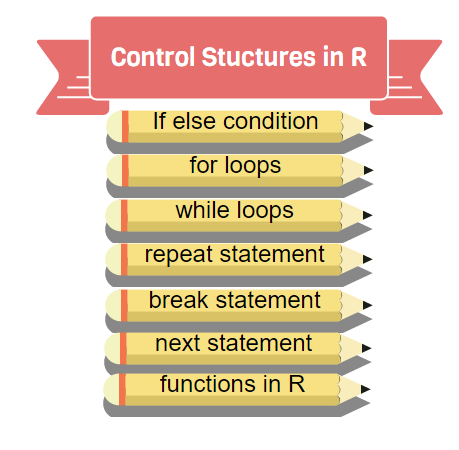
\includegraphics[width=0.7\linewidth]{control_structures+in+R} \end{center}

\href{https://www.r-bloggers.com/control-structures-loops-in-r/}{Control
Structures in R (R-Bloggers)}

\end{frame}

\begin{frame}{Breve repaso}
\protect\hypertarget{breve-repaso-2}{}


\includegraphics{bioconductor_logo_rgb.jpg}

\end{frame}

\begin{frame}{Breve repaso}
\protect\hypertarget{breve-repaso-3}{}

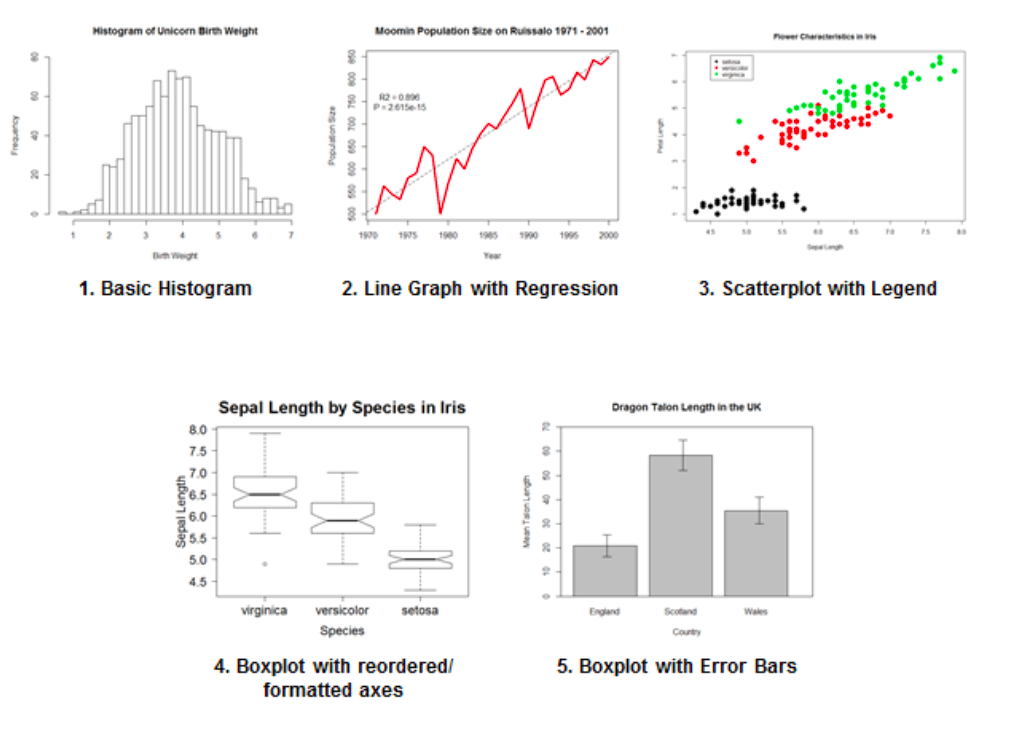
\includegraphics{r_base_graphs.png}

\href{https://rpubs.com/SusanEJohnston/7953}{R Base Graphs: an Idiot's
Guide}

\end{frame}

\begin{frame}{Análisis reproducible}
\protect\hypertarget{anuxe1lisis-reproducible}{}

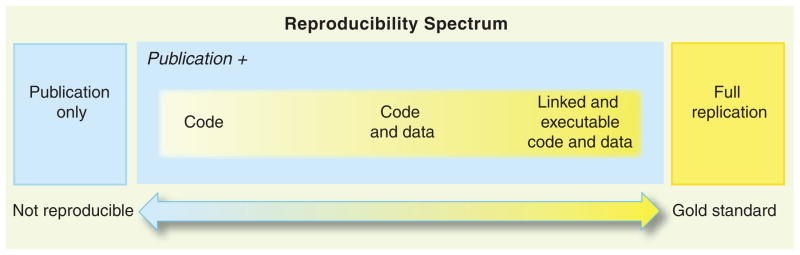
\includegraphics{gradiente_reproducibilidad.png}

\href{https://www.ncbi.nlm.nih.gov/pmc/articles/PMC3383002/}{Reproducible
Research in Computational Science (Peng, 2012)}

\end{frame}

\begin{frame}{Análisis reproducible}
\protect\hypertarget{anuxe1lisis-reproducible-1}{}

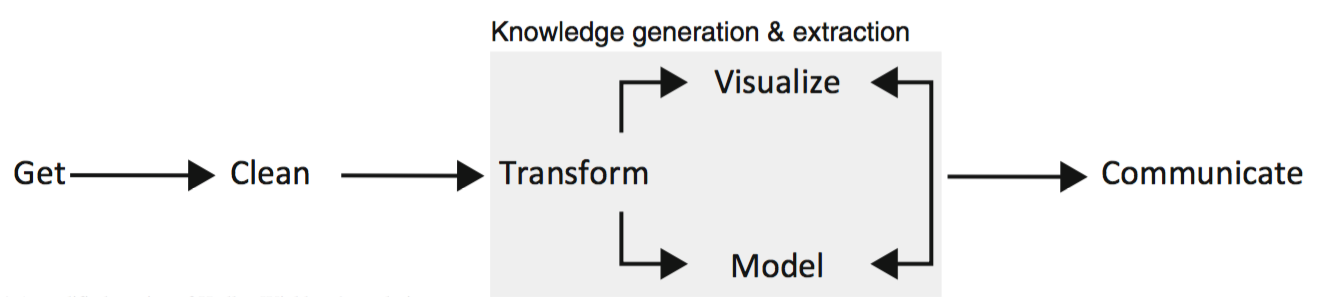
\includegraphics{analytic_process.png}

\href{http://93.174.95.29/_ads/6F902E466A32011DD94E2B6EEE505F9F}{Data
Wrangling with R (Boehmke, 2016)}

\end{frame}

\begin{frame}{Análisis reproducible en R}
\protect\hypertarget{anuxe1lisis-reproducible-en-r}{}

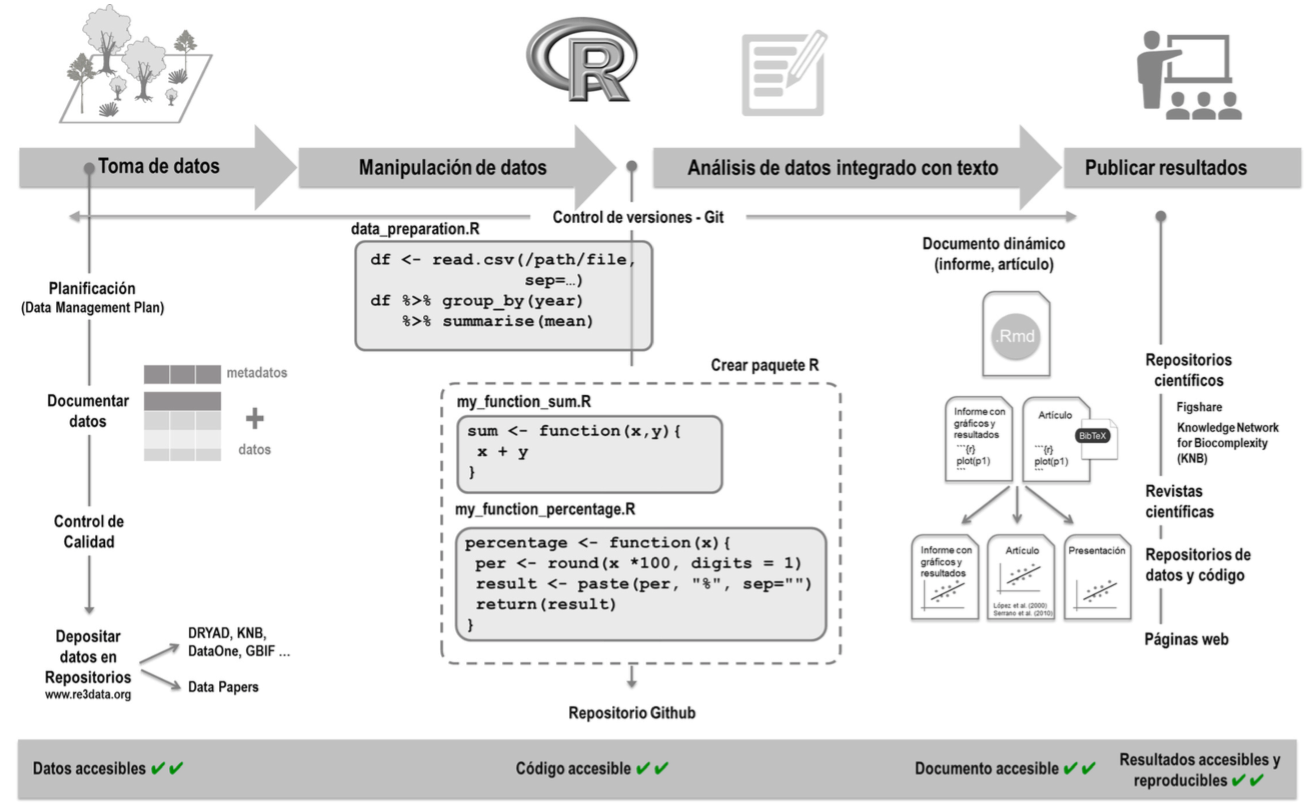
\includegraphics{analytic_process_R.png}

\href{}{Ciencia reproducible: qué, por qué, cómo (Rodríguez-Sánchez et
al., 2016)}

\end{frame}

\begin{frame}{Estructura de las clases}
\protect\hypertarget{estructura-de-las-clases}{}

\begin{itemize}
\tightlist
\item
  Teórico/práctico.
\item
  Práctico 11: repaso de loops y armado de funciones en R
\item
  Práctico 12: manejo de datos con paquetes de la librería
  \textbf{tidyverse}.
\end{itemize}

\end{frame}

\begin{frame}{Manejo de datos}
\protect\hypertarget{manejo-de-datos}{}

\begin{itemize}
\tightlist
\item
  \textbf{\emph{Data wrangling}}: es el proceso mediante el cual
  modificamos datos iniciales con el fin de analizarlos.
\end{itemize}

\end{frame}

\begin{frame}{Manejo de datos}
\protect\hypertarget{manejo-de-datos-1}{}

\begin{itemize}
\tightlist
\item
  \textbf{\emph{Data wrangling}}: es el proceso mediante el cual
  modificamos datos iniciales con el fin de analizarlos.
\item
  Incluye la edición, el filtrado, la obtención de nuevos y valores y
  más.
\end{itemize}

\end{frame}

\begin{frame}{Manejo de datos}
\protect\hypertarget{manejo-de-datos-2}{}

\begin{itemize}
\tightlist
\item
  \textbf{\emph{Data wrangling}}: es el proceso mediante el cual
  modificamos datos iniciales con el fin de analizarlos.
\item
  Incluye la edición, el filtrado, la obtención de nuevos y valores y
  más.
\item
  \emph{``In our experience, the tasks of exploratory data mining and
  data cleaning constitute 80\% of the effort that determines 80\% of
  the value of the ultimate data mining results. (\ldots{})''}.
  \textbf{Dasu \& Johnson.} \emph{Exploratory Data Mining and Data
  Cleaning} (2003).
\end{itemize}

\end{frame}

\begin{frame}{Manejo de datos}
\protect\hypertarget{manejo-de-datos-3}{}

Esto generalmente incluye

\begin{itemize}
\tightlist
\item
  Práctico 11

  \begin{itemize}
  \tightlist
  \item
    accionar sobre los datos para transformarlos: funciones
  \item
    realizar acciones repetitivas: loops
  \end{itemize}
\item
  Práctico 12

  \begin{itemize}
  \tightlist
  \item
    filtrado y edición de datos
  \item
    visualización de los datos
  \end{itemize}
\end{itemize}

\end{frame}

\hypertarget{funciones-en-r}{%
\section{Funciones en R}\label{funciones-en-r}}

\begin{frame}{Qué es una función?}
\protect\hypertarget{quuxe9-es-una-funciuxf3n}{}

\begin{itemize}
\tightlist
\item
  Un conjunto de \textbf{operaciones} definidas que toman
  \textbf{argumentos} para dar un resultado
\end{itemize}

\end{frame}

\begin{frame}{Funciones: una parte central de R}
\protect\hypertarget{funciones-una-parte-central-de-r}{}

\begin{itemize}
\tightlist
\item
  Es un lenguaje de programación en base a funciones: casi todo lo que
  hacemos las utiliza.

  \begin{itemize}
  \tightlist
  \item
    Otros lenguajes operan de forma diferente.
  \end{itemize}
\item
  R tiene funciones que vienen incorporadas por defecto
\item
  Utilizando librerías obtenemos nuevas funciones (como las de
  \textbf{seqinr}, por ejemplo)
\item
  Nosotros podemos hacer nuestras propias funciones
\end{itemize}

\end{frame}

\begin{frame}{Componentes de una función}
\protect\hypertarget{componentes-de-una-funciuxf3n}{}

\begin{itemize}
\tightlist
\item
  \textbf{cuerpo}: el código dentro de la función
\item
  \textbf{formales}: la lista de argumentos que controlan cómo se llama
  a la función
\item
  \textbf{ambiente}: el ``mapa'' de la locación de las variables de la
  función
\end{itemize}

\end{frame}

\begin{frame}[fragile]{Componentes de una función}
\protect\hypertarget{componentes-de-una-funciuxf3n-1}{}

\begin{Shaded}
\begin{Highlighting}[]
\KeywordTok{library}\NormalTok{(seqinr)}

\KeywordTok{body}\NormalTok{(seqinr}\OperatorTok{::}\NormalTok{GC)}
\end{Highlighting}
\end{Shaded}

\begin{verbatim}
## {
##     if (length(seq) == 1 && is.na(seq)) 
##         return(NA)
##     if (nchar(seq[1]) > 1) 
##         stop("sequence is not a vector of chars")
...
\end{verbatim}

\end{frame}

\begin{frame}[fragile]{Componentes de una función}
\protect\hypertarget{componentes-de-una-funciuxf3n-2}{}

\begin{Shaded}
\begin{Highlighting}[]
\KeywordTok{library}\NormalTok{(seqinr)}

\KeywordTok{formals}\NormalTok{(seqinr}\OperatorTok{::}\NormalTok{GC)}
\end{Highlighting}
\end{Shaded}

\begin{verbatim}
## $seq
## 
## 
## $forceToLower
## [1] TRUE
## 
## $exact
## [1] FALSE
## 
## $NA.GC
...
\end{verbatim}

\end{frame}

\begin{frame}[fragile]{Componentes de una función}
\protect\hypertarget{componentes-de-una-funciuxf3n-3}{}

\begin{Shaded}
\begin{Highlighting}[]
\KeywordTok{library}\NormalTok{(seqinr)}

\KeywordTok{environment}\NormalTok{(seqinr}\OperatorTok{::}\NormalTok{GC)}
\end{Highlighting}
\end{Shaded}

\begin{verbatim}
## <environment: namespace:seqinr>
\end{verbatim}

\end{frame}

\begin{frame}{Funciones particulares}
\protect\hypertarget{funciones-particulares}{}

\begin{itemize}
\tightlist
\item
  Podemos, además, distinguir tipos especiales de funciones:

  \begin{itemize}
  \tightlist
  \item
    \textbf{Funciones primitivas}: llaman directamente a C

    \begin{itemize}
    \tightlist
    \item
      No tienen cuerpo ni formales.
    \end{itemize}
  \item
    \textbf{Funciones de alto rango}: operan sobre funciones

    \begin{itemize}
    \tightlist
    \item
      Tienen cuerpo y formales, pero constituyen un caso interesante en
      sí
    \end{itemize}
  \end{itemize}
\end{itemize}

\end{frame}

\begin{frame}[fragile]{Funciones primitivas}
\protect\hypertarget{funciones-primitivas}{}

\begin{Shaded}
\begin{Highlighting}[]
\NormalTok{sum}
\end{Highlighting}
\end{Shaded}

\begin{verbatim}
## function (..., na.rm = FALSE)  .Primitive("sum")
\end{verbatim}

\begin{Shaded}
\begin{Highlighting}[]
\KeywordTok{body}\NormalTok{(sum)}
\end{Highlighting}
\end{Shaded}

\begin{verbatim}
## NULL
\end{verbatim}

\begin{Shaded}
\begin{Highlighting}[]
\KeywordTok{formals}\NormalTok{(sum)}
\end{Highlighting}
\end{Shaded}

\begin{verbatim}
## NULL
\end{verbatim}

\begin{Shaded}
\begin{Highlighting}[]
\KeywordTok{environment}\NormalTok{(sum)}
\end{Highlighting}
\end{Shaded}

\begin{verbatim}
## NULL
\end{verbatim}

\end{frame}

\begin{frame}[fragile]{Funciones primitivas}
\protect\hypertarget{funciones-primitivas-1}{}

\begin{Shaded}
\begin{Highlighting}[]
\StringTok{`}\DataTypeTok{[}\StringTok{`}
\end{Highlighting}
\end{Shaded}

\begin{verbatim}
## .Primitive("[")
\end{verbatim}

\begin{Shaded}
\begin{Highlighting}[]
\StringTok{`}\DataTypeTok{for}\StringTok{`}
\end{Highlighting}
\end{Shaded}

\begin{verbatim}
## .Primitive("for")
\end{verbatim}

\end{frame}

\begin{frame}[fragile]{Definición de funciones}
\protect\hypertarget{definiciuxf3n-de-funciones}{}

\begin{Shaded}
\begin{Highlighting}[]
\NormalTok{mi_funcion =}\StringTok{ }\ControlFlowTok{function}\NormalTok{(argumento_}\DecValTok{1}\NormalTok{, argumento_}\DecValTok{2}\NormalTok{, ...)\{}
  \CommentTok{# en este bloque suceden operaciones con argumento_1}
\NormalTok{  ...}
  \CommentTok{# en este bloque suceden operaciones con argumento_2}
\NormalTok{  ...}
  \CommentTok{# se devuelve algo como resultado de aplicar}
  \CommentTok{# la funcion a los argumentos}
  \KeywordTok{return}\NormalTok{(una_variable_nueva)}
\NormalTok{\}}
\end{Highlighting}
\end{Shaded}

\end{frame}

\begin{frame}[fragile]{Definición de funciones}
\protect\hypertarget{definiciuxf3n-de-funciones-1}{}

\begin{Shaded}
\begin{Highlighting}[]
\NormalTok{eleva_y_resta =}\StringTok{ }\ControlFlowTok{function}\NormalTok{(x,y)\{}
\NormalTok{  resultado =}\StringTok{ }\NormalTok{x}\OperatorTok{^}\DecValTok{2} \OperatorTok{-}\StringTok{ }\NormalTok{y}\OperatorTok{^}\DecValTok{2}
  \KeywordTok{return}\NormalTok{(resultado)}
\NormalTok{\}}
\end{Highlighting}
\end{Shaded}

\end{frame}

\begin{frame}[fragile]{Definición de funciones}
\protect\hypertarget{definiciuxf3n-de-funciones-2}{}

\begin{Shaded}
\begin{Highlighting}[]
\NormalTok{eleva_y_resta =}\StringTok{ }\ControlFlowTok{function}\NormalTok{(x,y)\{}
\NormalTok{  resultado =}\StringTok{ }\NormalTok{x}\OperatorTok{^}\DecValTok{2} \OperatorTok{-}\StringTok{ }\NormalTok{y}\OperatorTok{^}\DecValTok{2}
  \KeywordTok{return}\NormalTok{(resultado)}
\NormalTok{\}}

\KeywordTok{eleva_y_resta}\NormalTok{(}\DecValTok{2}\NormalTok{,}\DecValTok{3}\NormalTok{)}
\end{Highlighting}
\end{Shaded}

\begin{verbatim}
## [1] -5
\end{verbatim}

\end{frame}

\begin{frame}[fragile]{Definición de funciones}
\protect\hypertarget{definiciuxf3n-de-funciones-3}{}

\begin{Shaded}
\begin{Highlighting}[]
\NormalTok{eleva_y_resta =}\StringTok{ }\ControlFlowTok{function}\NormalTok{(x,y)\{}
\NormalTok{  resultado =}\StringTok{ }\NormalTok{x}\OperatorTok{^}\DecValTok{2} \OperatorTok{+}\StringTok{ }\NormalTok{y}\OperatorTok{^}\DecValTok{2}
  \KeywordTok{return}\NormalTok{(resultado)}
\NormalTok{\}}

\KeywordTok{eleva_y_resta}\NormalTok{(}\DataTypeTok{y =} \DecValTok{2}\NormalTok{, }\DataTypeTok{x =}\DecValTok{3}\NormalTok{)}
\end{Highlighting}
\end{Shaded}

\begin{verbatim}
## [1] 13
\end{verbatim}

\end{frame}

\begin{frame}[fragile]{Definición de funciones}
\protect\hypertarget{definiciuxf3n-de-funciones-4}{}

\begin{Shaded}
\begin{Highlighting}[]
\NormalTok{eleva_y_resta =}\StringTok{ }\ControlFlowTok{function}\NormalTok{(x,y)\{}
\NormalTok{  resultado =}\StringTok{ }\NormalTok{x}\OperatorTok{^}\DecValTok{2} \OperatorTok{-}\StringTok{ }\NormalTok{y}\OperatorTok{^}\DecValTok{2}
  \KeywordTok{return}\NormalTok{(resultado)}
\NormalTok{\}}

\KeywordTok{eleva_y_resta}\NormalTok{(}\DataTypeTok{y =} \DecValTok{2}\NormalTok{)}
\end{Highlighting}
\end{Shaded}

\begin{verbatim}
## Error in eleva_y_resta(y = 2): argument "x" is missing, with no default
\end{verbatim}

\end{frame}

\begin{frame}[fragile]{Definición de funciones}
\protect\hypertarget{definiciuxf3n-de-funciones-5}{}

\begin{Shaded}
\begin{Highlighting}[]
\NormalTok{eleva_y_resta =}\StringTok{ }\ControlFlowTok{function}\NormalTok{(}\DataTypeTok{x =} \DecValTok{1}\NormalTok{, }\DataTypeTok{y =}\DecValTok{1}\NormalTok{)\{}
\NormalTok{  resultado =}\StringTok{ }\NormalTok{x}\OperatorTok{^}\DecValTok{2} \OperatorTok{-}\StringTok{ }\NormalTok{y}\OperatorTok{^}\DecValTok{2}
  \KeywordTok{return}\NormalTok{(resultado)}
\NormalTok{\}}

\KeywordTok{eleva_y_resta}\NormalTok{(}\DataTypeTok{y =} \DecValTok{2}\NormalTok{)}
\end{Highlighting}
\end{Shaded}

\begin{verbatim}
## [1] -3
\end{verbatim}

\end{frame}

\begin{frame}[fragile]{Definición de funciones}
\protect\hypertarget{definiciuxf3n-de-funciones-6}{}

\begin{Shaded}
\begin{Highlighting}[]
\CommentTok{# ojo con el alcance de las variables!}
\NormalTok{x =}\StringTok{ }\DecValTok{2}
\NormalTok{eleva_y_resta =}\StringTok{ }\ControlFlowTok{function}\NormalTok{(x, y)\{}
\NormalTok{  resultado =}\StringTok{ }\NormalTok{x}\OperatorTok{^}\DecValTok{2} \OperatorTok{-}\StringTok{ }\NormalTok{y}\OperatorTok{^}\DecValTok{2}
  \KeywordTok{return}\NormalTok{(resultado)}
\NormalTok{\}}

\KeywordTok{eleva_y_resta}\NormalTok{(}\DataTypeTok{y =} \DecValTok{2}\NormalTok{)}
\end{Highlighting}
\end{Shaded}

\begin{verbatim}
## [1] 0
\end{verbatim}

\end{frame}

\begin{frame}[fragile]{Programación defensiva}
\protect\hypertarget{programaciuxf3n-defensiva}{}

\begin{itemize}
\tightlist
\item
  la función \textbf{stop()} permite salir de la función si algo
  esperable no sucede
\end{itemize}

\small

\begin{Shaded}
\begin{Highlighting}[]
\NormalTok{eleva_y_resta =}\StringTok{ }\ControlFlowTok{function}\NormalTok{(}\DataTypeTok{x =} \DecValTok{1}\NormalTok{, }\DataTypeTok{y =}\DecValTok{1}\NormalTok{)\{}
  
  \ControlFlowTok{if}\NormalTok{(}\OperatorTok{!}\KeywordTok{is.numeric}\NormalTok{(x) }\OperatorTok{|}\StringTok{ }\OperatorTok{!}\KeywordTok{is.numeric}\NormalTok{(y))\{}
    \KeywordTok{stop}\NormalTok{(}\StringTok{'Alguno de los argumentos dados no es un numero.'}\NormalTok{)}
\NormalTok{  \}}
  
\NormalTok{  resultado =}\StringTok{ }\NormalTok{x}\OperatorTok{^}\DecValTok{2} \OperatorTok{-}\StringTok{ }\NormalTok{y}\OperatorTok{^}\DecValTok{2}
  \KeywordTok{return}\NormalTok{(resultado)}
\NormalTok{\}}

\KeywordTok{eleva_y_resta}\NormalTok{(}\DataTypeTok{x =} \DecValTok{2}\NormalTok{, }\DataTypeTok{y =} \StringTok{"2"}\NormalTok{)}
\end{Highlighting}
\end{Shaded}

\begin{verbatim}
## Error in eleva_y_resta(x = 2, y = "2"): Alguno de los argumentos dados no es un numero.
\end{verbatim}

\normalsize

\end{frame}

\begin{frame}[fragile]{Salida de funciones}
\protect\hypertarget{salida-de-funciones}{}

\begin{Shaded}
\begin{Highlighting}[]
\CommentTok{# ojo con el alcance de las variables!}
\NormalTok{x =}\StringTok{ }\DecValTok{2}
\NormalTok{eleva_resta_y_suma =}\StringTok{ }\ControlFlowTok{function}\NormalTok{(x, y)\{}
\NormalTok{  resta =}\StringTok{ }\NormalTok{x}\OperatorTok{^}\DecValTok{2} \OperatorTok{-}\StringTok{ }\NormalTok{y}\OperatorTok{^}\DecValTok{2}
\NormalTok{  suma =}\StringTok{ }\NormalTok{x}\OperatorTok{^}\DecValTok{2} \OperatorTok{+}\StringTok{ }\NormalTok{y}\OperatorTok{^}\DecValTok{2}
  \KeywordTok{return}\NormalTok{(}\KeywordTok{c}\NormalTok{(resta, suma))}
\NormalTok{\}}

\KeywordTok{eleva_resta_y_suma}\NormalTok{(}\DataTypeTok{x =} \DecValTok{2}\NormalTok{, }\DataTypeTok{y =} \DecValTok{2}\NormalTok{)}
\end{Highlighting}
\end{Shaded}

\begin{verbatim}
## [1] 0 8
\end{verbatim}

\end{frame}

\begin{frame}[fragile]{Salida de funciones}
\protect\hypertarget{salida-de-funciones-1}{}

\begin{Shaded}
\begin{Highlighting}[]
\CommentTok{# ojo con el alcance de las variables!}
\NormalTok{x =}\StringTok{ }\DecValTok{2}
\NormalTok{eleva_resta_y_suma =}\StringTok{ }\ControlFlowTok{function}\NormalTok{(x, y)\{}
\NormalTok{  resta =}\StringTok{ }\NormalTok{x}\OperatorTok{^}\DecValTok{2} \OperatorTok{-}\StringTok{ }\NormalTok{y}\OperatorTok{^}\DecValTok{2}
\NormalTok{  suma =}\StringTok{ }\NormalTok{x}\OperatorTok{^}\DecValTok{2} \OperatorTok{+}\StringTok{ }\NormalTok{y}\OperatorTok{^}\DecValTok{2}
  \KeywordTok{return}\NormalTok{(}\KeywordTok{c}\NormalTok{(}\KeywordTok{list}\NormalTok{(resta, suma)))}
\NormalTok{\}}

\KeywordTok{eleva_resta_y_suma}\NormalTok{(}\DataTypeTok{x =} \DecValTok{2}\NormalTok{, }\DataTypeTok{y =} \DecValTok{2}\NormalTok{)}
\end{Highlighting}
\end{Shaded}

\begin{verbatim}
## [[1]]
## [1] 0
## 
## [[2]]
## [1] 8
\end{verbatim}

\end{frame}

\begin{frame}{Funciones de alto rango (\emph{high-order functions})}
\protect\hypertarget{funciones-de-alto-rango-high-order-functions}{}

\begin{itemize}
\tightlist
\item
  Son funciones que toman a otras funciones como argumentos y devuelven
  una función o valor.
\item
  Funciones como apply(), sapply(), lapply(), mapply()\ldots{}
\end{itemize}

\end{frame}

\begin{frame}[fragile]{sapply}
\protect\hypertarget{sapply}{}

\small

\begin{Shaded}
\begin{Highlighting}[]
\CommentTok{# definimos un vector}
\NormalTok{numeros =}\StringTok{ }\KeywordTok{c}\NormalTok{(}\DecValTok{1}\NormalTok{,}\DecValTok{2}\NormalTok{,}\DecValTok{3}\NormalTok{,}\DecValTok{4}\NormalTok{)}

\CommentTok{# aplicamos una funcion anonima sobre este vector}
\NormalTok{numeros_cuadrado =}\StringTok{ }\KeywordTok{sapply}\NormalTok{(}\DataTypeTok{X =}\NormalTok{ numeros, }\DataTypeTok{FUN =} \ControlFlowTok{function}\NormalTok{(x)\{x}\OperatorTok{^}\DecValTok{2}\NormalTok{\})}

\NormalTok{numeros_cuadrado}
\end{Highlighting}
\end{Shaded}

\begin{verbatim}
## [1]  1  4  9 16
\end{verbatim}

\normalsize

\end{frame}

\begin{frame}[fragile]{lapply}
\protect\hypertarget{lapply}{}

\small

\begin{Shaded}
\begin{Highlighting}[]
\CommentTok{# definimos un vector}
\NormalTok{numeros =}\StringTok{ }\KeywordTok{c}\NormalTok{(}\DecValTok{1}\NormalTok{,}\DecValTok{2}\NormalTok{,}\DecValTok{3}\NormalTok{,}\DecValTok{4}\NormalTok{)}

\CommentTok{# aplicamos una funcion anonima sobre este vector}
\NormalTok{numeros_cuadrado =}\StringTok{ }\KeywordTok{lapply}\NormalTok{(}\DataTypeTok{X =}\NormalTok{ numeros, }\DataTypeTok{FUN =} \ControlFlowTok{function}\NormalTok{(x)\{x}\OperatorTok{^}\DecValTok{2}\NormalTok{\})}

\NormalTok{numeros_cuadrado}
\end{Highlighting}
\end{Shaded}

\begin{verbatim}
## [[1]]
## [1] 1
## 
## [[2]]
## [1] 4
...
\end{verbatim}

\normalsize

\end{frame}

\begin{frame}[fragile]{mapply}
\protect\hypertarget{mapply}{}

\begin{Shaded}
\begin{Highlighting}[]
\CommentTok{# creando una matriz de 4x4 con mapply}
\NormalTok{matriz =}\StringTok{ }\KeywordTok{mapply}\NormalTok{(rep, }\DecValTok{1}\OperatorTok{:}\DecValTok{4}\NormalTok{, }\DecValTok{4}\NormalTok{)}

\NormalTok{matriz}
\end{Highlighting}
\end{Shaded}

\begin{verbatim}
##      [,1] [,2] [,3] [,4]
## [1,]    1    2    3    4
## [2,]    1    2    3    4
## [3,]    1    2    3    4
## [4,]    1    2    3    4
\end{verbatim}

\end{frame}

\hypertarget{loops-en-r}{%
\section{Loops en R}\label{loops-en-r}}

\begin{frame}[fragile]{For loop (abstracto)}
\protect\hypertarget{for-loop-abstracto}{}

\begin{Shaded}
\begin{Highlighting}[]
\CommentTok{# for loop}

\NormalTok{un_vector =}\StringTok{ }\NormalTok{...}
\ControlFlowTok{for}\NormalTok{ (i }\ControlFlowTok{in}\NormalTok{ ____) \{}
\NormalTok{  ...}
\NormalTok{  ... un_vector[i] ....}
\NormalTok{  ...}
\NormalTok{\}}
\end{Highlighting}
\end{Shaded}

\end{frame}

\begin{frame}[fragile]{For loop (ejemplo)}
\protect\hypertarget{for-loop-ejemplo}{}

\begin{Shaded}
\begin{Highlighting}[]
\NormalTok{numeros =}\StringTok{ }\KeywordTok{c}\NormalTok{(}\DecValTok{3}\NormalTok{,}\DecValTok{40}\NormalTok{,}\DecValTok{15}\NormalTok{,}\DecValTok{6}\NormalTok{)}
\NormalTok{numeros_cuadrado =}\StringTok{ }\KeywordTok{c}\NormalTok{()}

\ControlFlowTok{for}\NormalTok{ (i }\ControlFlowTok{in} \DecValTok{1}\OperatorTok{:}\KeywordTok{length}\NormalTok{(numeros)) \{}
\NormalTok{  numeros_cuadrado[i] =}\StringTok{ }\NormalTok{numeros[i]}\OperatorTok{^}\DecValTok{2}
\NormalTok{\}}
\end{Highlighting}
\end{Shaded}

\end{frame}

\begin{frame}[fragile]{For loop (usando seq\_along())}
\protect\hypertarget{for-loop-usando-seq_along}{}

\begin{Shaded}
\begin{Highlighting}[]
\NormalTok{numeros =}\StringTok{ }\KeywordTok{c}\NormalTok{(}\DecValTok{3}\NormalTok{,}\DecValTok{40}\NormalTok{,}\DecValTok{15}\NormalTok{,}\DecValTok{6}\NormalTok{)}
\NormalTok{numeros_cuadrado =}\StringTok{ }\KeywordTok{c}\NormalTok{()}

\ControlFlowTok{for}\NormalTok{ (i }\ControlFlowTok{in} \KeywordTok{seq_along}\NormalTok{(numeros)) \{}
\NormalTok{  numeros_cuadrado[i] =}\StringTok{ }\NormalTok{numeros[i]}\OperatorTok{^}\DecValTok{2}
\NormalTok{\}}
\end{Highlighting}
\end{Shaded}

\end{frame}

\begin{frame}[fragile]{Operador next}
\protect\hypertarget{operador-next}{}

\begin{Shaded}
\begin{Highlighting}[]
\NormalTok{numeros =}\StringTok{ }\KeywordTok{c}\NormalTok{(}\DecValTok{3}\NormalTok{,}\DecValTok{40}\NormalTok{,}\DecValTok{15}\NormalTok{,}\DecValTok{6}\NormalTok{)}
\NormalTok{numeros_cuadrado =}\StringTok{ }\KeywordTok{c}\NormalTok{()}

\ControlFlowTok{for}\NormalTok{ (i }\ControlFlowTok{in} \KeywordTok{seq_along}\NormalTok{(numeros)) \{}
  
  \ControlFlowTok{if}\NormalTok{(}\OperatorTok{!}\NormalTok{numeros[i] }\OperatorTok\StringTok{ }\DecValTok{3} \OperatorTok{==}\StringTok{ }\DecValTok{0}\NormalTok{)\{}
    \ControlFlowTok{next}
\NormalTok{  \}}
  \ControlFlowTok{else}\NormalTok{ \{}
\NormalTok{  numeros_cuadrado[i] =}\StringTok{ }\NormalTok{numeros[i]}\OperatorTok{^}\DecValTok{2}
\NormalTok{  \}}
\NormalTok{\}}
\NormalTok{numeros_cuadrado}
\end{Highlighting}
\end{Shaded}

\begin{verbatim}
## [1]   9  NA 225  36
\end{verbatim}

\end{frame}

\begin{frame}[fragile]{Operador break}
\protect\hypertarget{operador-break}{}

\begin{Shaded}
\begin{Highlighting}[]
\NormalTok{numeros =}\StringTok{ }\KeywordTok{c}\NormalTok{(}\DecValTok{3}\NormalTok{,}\DecValTok{40}\NormalTok{,}\DecValTok{15}\NormalTok{,}\DecValTok{6}\NormalTok{)}
\NormalTok{numeros_cuadrado =}\StringTok{ }\KeywordTok{c}\NormalTok{()}

\ControlFlowTok{for}\NormalTok{ (i }\ControlFlowTok{in} \KeywordTok{seq_along}\NormalTok{(numeros)) \{}
  
  \ControlFlowTok{if}\NormalTok{(}\OperatorTok{!}\NormalTok{numeros[i] }\OperatorTok\StringTok{ }\DecValTok{3} \OperatorTok{==}\StringTok{ }\DecValTok{0}\NormalTok{)\{}
    \ControlFlowTok{break}
\NormalTok{  \}}
  
\NormalTok{  numeros_cuadrado[i] =}\StringTok{ }\NormalTok{numeros[i]}\OperatorTok{^}\DecValTok{2}
\NormalTok{\}}
\NormalTok{numeros_cuadrado}
\end{Highlighting}
\end{Shaded}

\begin{verbatim}
## [1] 9
\end{verbatim}

\end{frame}

\begin{frame}{While loop}
\protect\hypertarget{while-loop}{}

\begin{itemize}
\tightlist
\item
  Sigue la misma lógica que en Bash
\item
  Se utiliza la función while() en vez de for()
\item
  Se puede realizar combinando un for loop con un operador break
\end{itemize}

\end{frame}

\end{document}
